\documentclass[spanish,letterpaper,oneside]{article}

% Datos del documento
\def\documenttitle {Multiplicación, división y números con signo}
\def\documentsubtitle {Temas selectos de matemáticas I}
\def\documentsubject {Actividad 3 · Dos fichas oficiales resueltas}
\def\documentauthor {Mtro. Martín Jonathan de la Cruz Muñoz}
\def\coursename {Temas selectos de matemáticas I}
\def\coursecode {PFM02}

% Identidad institucional
\def\universityname {Instituto de Investigación, Innovación y Estudios de Posgrado para la Educación del Estado de Nuevo León}
\def\universityfaculty {Maestría en Aprendizaje y Enseñanza de las Matemáticas}
\def\universitydepartment {Temas selectos de matemáticas I}
\def\universitydepartmentimage {img/iiiepe/marca-iiiepe.png}
\def\universitydepartmentimagecfg {height=1.75cm}
\def\universitylocation {Monterrey, Nuevo León}
\def\studentfullname {Mtro. Martín Jonathan de la Cruz Muñoz}
\def\studentid {00874}
\def\studentemail {martin.delacruz@campus.iiiepe.edu.mx}
\def\programperiod {1er tetramestre, marzo--julio de 2026}
\def\programmodality {Modalidad presencial}
\def\programshort {MAEM}

\def\authortable {
  \begin{tabular}{ll}
    \textbf{Alumno:} & \studentfullname \\
    Matrícula: & \studentid \\
    Correo institucional: & \studentemail \\
    Unidad: & \coursename \\
    Programa: & \programshort \\
    Periodo: & \programperiod \\
    & \\
    \multicolumn{2}{l}{Fecha de realización: 13 de octubre de 2026} \\
    \multicolumn{2}{l}{\universitylocation}
  \end{tabular}
}

\input{template}

\usepackage{helvet}
\renewcommand{\familydefault}{\sfdefault}
\usepackage{array}
\usepackage{longtable}
\usepackage{pdflscape}
\usepackage{tikz}
\usepackage[most]{tcolorbox}
\usetikzlibrary{arrows.meta,positioning,calc,fit,backgrounds}

\definecolor{iiiepeNavy}{HTML}{163B5C}
\definecolor{iiiepeBlue}{HTML}{1F6F9F}
\definecolor{iiiepeAqua}{HTML}{20B7A8}
\definecolor{iiiepeOrange}{HTML}{F28C28}
\definecolor{iiiepePaper}{HTML}{F6F8F7}
\definecolor{iiiepeInk}{HTML}{1E2A32}
\def\portraittitlecolor {iiiepeNavy}
\setcitestyle{authoryear,open={(},close={)}}

\newcommand{\insertcoverwatermark}{%
  \AddToShipoutPictureBG*{%
    \begin{tikzpicture}[remember picture,overlay]
      \node[opacity=.09,inner sep=0pt] at (current page.center)
      {\includegraphics[width=.58\paperwidth]{img/iiiepe/logo-puntos.png}};
    \end{tikzpicture}%
  }%
}

\newtcolorbox{reportelecturabox}[1][]{%
  enhanced,breakable,
  colback=iiiepePaper,colframe=iiiepeNavy,
  boxrule=1pt,leftrule=4pt,arc=2pt,
  left=8pt,right=8pt,top=6pt,bottom=6pt,
  before skip=6pt,after skip=10pt,
  fonttitle=\bfseries\color{white},coltitle=white,
  colbacktitle=iiiepeNavy,
  attach boxed title to top left={xshift=8pt,yshift=-2pt},
  boxed title style={colback=iiiepeNavy,colframe=iiiepeNavy,arc=1pt},
  title={Reporte de lectura},#1}

\newtcolorbox{fichalecturabox}[1][]{%
  enhanced,breakable,
  colback=iiiepeAqua!7,colframe=iiiepeAqua!70!iiiepeNavy,
  boxrule=.6pt,arc=1pt,
  left=7pt,right=7pt,top=4pt,bottom=4pt,
  fontupper=\small,before upper={\setstretch{1.0}},
  fonttitle=\bfseries\color{iiiepeNavy},coltitle=iiiepeNavy,
  colbacktitle=iiiepeAqua!7,
  title={Ficha de la lectura},#1}



\usepackage{tabularx,colortbl,pgfplots,enumitem,needspace}\pgfplotsset{compat=1.18}\definecolor{iiiepePale}{HTML}{EEF5F8}
\setlength{\parskip}{5pt}\setlength{\parindent}{0pt}
\begin{document}\insertcoverwatermark\templatePortrait\templatePagecfg\templateFinalcfg\fancyfoot{}\fancyfoot[L]{\scriptsize IIIEPE · MAEM}\fancyfoot[C]{\scriptsize\thepage}\fancyfoot[R]{\scriptsize Actividad 3}\setstretch{1.3}\raggedbottom
\section{Operar y justificar el significado}
Multiplicar fracciones permite calcular una parte de otra cantidad; dividir permite medir cuántas porciones del tamaño indicado caben en una cantidad. Los signos incorporan dirección, deuda o posición respecto de una referencia. En el taller, una operación debe conservar unidades y significado: un resultado numéricamente correcto puede ser inadecuado si confunde área, longitud o número de piezas.
\[
\frac ab\frac cd=\frac{ac}{bd},\qquad \frac ab\div\frac cd=\frac{ad}{bc},\quad b,c,d\ne0.
\]
Dividir por $c/d$ equivale a multiplicar por $d/c$ porque su producto es 1. Se invierte únicamente el divisor. Los números mixtos se convierten a fracciones impropias antes de operar.

\begin{center}
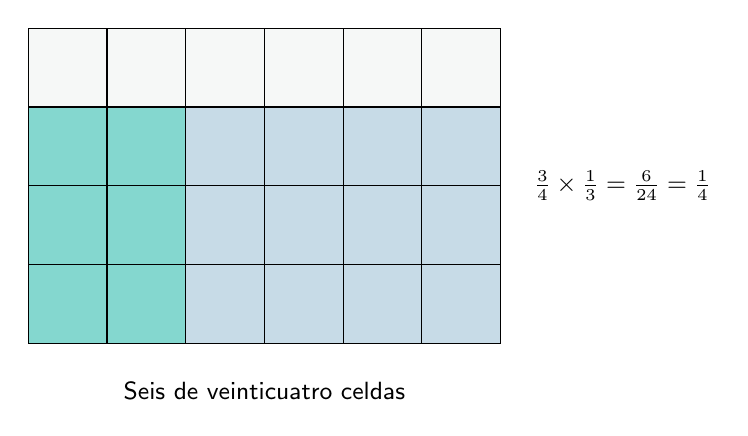
\begin{tikzpicture}[x=1cm,y=1cm,font=\small]
\draw[fill=iiiepePaper] (0,0) rectangle (6,4);\fill[iiiepeBlue!25] (0,0) rectangle (6,3);\fill[iiiepeAqua!55] (0,0) rectangle (2,3);
\foreach \x in {0,1,2,3,4,5,6}\draw (\x,0)--(\x,4);\foreach \y in {0,1,2,3,4}\draw (0,\y)--(6,\y);
\node[right] at (6.3,2){$\frac34\times\frac13=\frac6{24}=\frac14$};\node at (3,-.6){Seis de veinticuatro celdas};\end{tikzpicture}
\end{center}
\section{Sesión 03 A · Fracciones}
\subsection*{Multiplicaciones}


{\small\setstretch{1.1}\renewcommand{\arraystretch}{1.25}
\begin{longtable}{|>{\raggedright\arraybackslash}p{\dimexpr0.5\linewidth-2\tabcolsep-2\arrayrulewidth\relax}|>{\raggedright\arraybackslash}p{\dimexpr0.5\linewidth-2\tabcolsep-2\arrayrulewidth\relax}|}\hline
\rowcolor{iiiepePale} \textbf{Expresión} & \textbf{Procedimiento y resultado} \\\hline
\endfirsthead
\hline
\rowcolor{iiiepePale} \textbf{Expresión} & \textbf{Procedimiento y resultado} \\\hline
\endhead
$\frac{3}{4}\times \frac{5}{9}$ & $\frac{5}{12}$ \\\hline
$\frac{4}{9}\times \frac{12}{7}$ & $\frac{16}{21}$ \\\hline
$\frac{23}{25}\times \frac{6}{5}$ & $\frac{138}{125}$ \\\hline
$7\times \frac{3}{11}$ & $\frac{21}{11}$ \\\hline
$\frac{17}{5}\times \frac{8}{7}$ & $\frac{136}{35}$ \\\hline
$\frac34\frac25\frac69$ & $\frac{36}{180}=\frac15$ \\\hline
\end{longtable}}

\subsection*{Divisiones}


{\small\setstretch{1.1}\renewcommand{\arraystretch}{1.25}
\begin{longtable}{|>{\raggedright\arraybackslash}p{\dimexpr0.5\linewidth-2\tabcolsep-2\arrayrulewidth\relax}|>{\raggedright\arraybackslash}p{\dimexpr0.5\linewidth-2\tabcolsep-2\arrayrulewidth\relax}|}\hline
\rowcolor{iiiepePale} \textbf{Expresión} & \textbf{Procedimiento y resultado} \\\hline
\endfirsthead
\hline
\rowcolor{iiiepePale} \textbf{Expresión} & \textbf{Procedimiento y resultado} \\\hline
\endhead
$\frac{7}{8}\div \frac{1}{6}$ & $\frac{7}{8}\times 6=\frac{21}{4}$ \\\hline
$\frac{5}{7}\div \frac{1}{3}$ & $\frac{5}{7}\times 3=\frac{15}{7}$ \\\hline
$\frac{2}{7}\div \frac{6}{7}$ & $\frac{2}{7}\times \frac{7}{6}=\frac{1}{3}$ \\\hline
$\frac{9}{7}\div \frac{21}{8}$ & $\frac{9}{7}\times \frac{8}{21}=\frac{24}{49}$ \\\hline
$\frac{5}{6}\div \frac{2}{3}$ & $\frac{5}{6}\times \frac{3}{2}=\frac{5}{4}$ \\\hline
$\frac{3}{4}\div \frac{2}{5}$ & $\frac{3}{4}\times \frac{5}{2}=\frac{15}{8}$ \\\hline
$\frac{8}{9}\div \frac{3}{2}$ & $\frac{8}{9}\times \frac{2}{3}=\frac{16}{27}$ \\\hline
\end{longtable}}

\subsection*{Situaciones contextualizadas}

{\small\setstretch{1.1}\renewcommand{\arraystretch}{1.25}
\begin{longtable}{|>{\raggedright\arraybackslash}p{\dimexpr0.22\linewidth-2\tabcolsep-2\arrayrulewidth\relax}|>{\raggedright\arraybackslash}p{\dimexpr0.78\linewidth-2\tabcolsep-2\arrayrulewidth\relax}|}\hline
\rowcolor{iiiepePale} \textbf{Caso} & \textbf{Operación y respuesta} \\\hline
\endfirsthead
\hline
\rowcolor{iiiepePale} \textbf{Caso} & \textbf{Operación y respuesta} \\\hline
\endhead
1a & Si la producción anual es constante $P$, de 2023 a 2030 inclusive hay ocho años: $8P/3$. Es el equivalente a $2\frac23$ producciones anuales, no una masa determinada porque el enunciado no proporciona toneladas. \\\hline
1b & La mitad del desperdicio $P/3$ es $P/6$. La meta es desperdiciar como máximo una sexta parte de la producción anual, bajo ese supuesto. \\\hline
2a & $3(12)(3/4)=27$ litros de jugo. \\\hline
2b & La mitad de $3/4$ m$^2$ es $(1/2)(3/4)=3/8$ m$^2$. \\\hline
3 & Deuda $=(3/4)(132)=99$ pesos; pago $=(2/3)(99)=66$; saldo $99-66=33$ pesos. \\\hline
4 & $4\frac34\div1/4=(19/4)(4)=19$ varillas, sin considerar pérdidas de corte. \\\hline
\end{longtable}}



{\small\setstretch{1.1}\renewcommand{\arraystretch}{1.25}
\begin{longtable}{|>{\raggedright\arraybackslash}p{\dimexpr0.22\linewidth-2\tabcolsep-2\arrayrulewidth\relax}|>{\raggedright\arraybackslash}p{\dimexpr0.78\linewidth-2\tabcolsep-2\arrayrulewidth\relax}|}\hline
\rowcolor{iiiepePale} \textbf{Caso} & \textbf{Operación y respuesta} \\\hline
\endfirsthead
\hline
\rowcolor{iiiepePale} \textbf{Caso} & \textbf{Operación y respuesta} \\\hline
\endhead
5 & Venta: $(2/5)(20)=8$ ha. Restan 12; alquiler: $(3/4)(12)=9$ ha; quedan $12-9=3$ ha sin vender ni alquilar. \\\hline
6 & Ancho $=A/l=(21/4)/(7/2)=(21/4)(2/7)=3/2$ m. \\\hline
7 & Área del rectángulo $=(13/7)(4/5)=52/35$ unidades cuadradas. \\\hline
8 & $(32\frac15)/(1\frac25)=(161/5)/(7/5)=23$ botellas completas. \\\hline
9 & $(11\frac14)/(3/4)=(45/4)(4/3)=15$ vasos. \\\hline
10 & $(3/4)(4\frac23)=(3/4)(14/3)=7/2=42/12$ kg; opción a. \\\hline
11 & $1\frac12\div1/10=(3/2)(10)=15$ bolsas. \\\hline
\end{longtable}}

\section{Sesión 03 B · Números negativos}
El simétrico de $a$ es $-a$ y su suma es cero. El valor absoluto $|a|$ mide distancia al cero y nunca es negativo. En sumas se combinan posiciones o cambios; en productos, dos signos negativos producen uno positivo por consistencia con la propiedad distributiva.
\subsection*{Simétricos}


{\small\setstretch{1.1}\renewcommand{\arraystretch}{1.25}
\begin{longtable}{|>{\raggedright\arraybackslash}p{\dimexpr0.5\linewidth-2\tabcolsep-2\arrayrulewidth\relax}|>{\raggedright\arraybackslash}p{\dimexpr0.5\linewidth-2\tabcolsep-2\arrayrulewidth\relax}|}\hline
\rowcolor{iiiepePale} \textbf{Expresión} & \textbf{Procedimiento y resultado} \\\hline
\endfirsthead
\hline
\rowcolor{iiiepePale} \textbf{Expresión} & \textbf{Procedimiento y resultado} \\\hline
\endhead
$9$ & $-(9)=-9$ \\\hline
$-6$ & $-(-6)=6$ \\\hline
$13$ & $-(13)=-13$ \\\hline
$1/8$ & $-(1/8)=-1/8$ \\\hline
$-5/4$ & $-(-5/4)=5/4$ \\\hline
$0$ & $-(0)=0$ \\\hline
$0.25$ & $-(0.25)=-1/4$ \\\hline
$-12.5$ & $-(-12.5)=25/2$ \\\hline
\end{longtable}}

\subsection*{Valores absolutos}


{\small\setstretch{1.1}\renewcommand{\arraystretch}{1.25}
\begin{longtable}{|>{\raggedright\arraybackslash}p{\dimexpr0.5\linewidth-2\tabcolsep-2\arrayrulewidth\relax}|>{\raggedright\arraybackslash}p{\dimexpr0.5\linewidth-2\tabcolsep-2\arrayrulewidth\relax}|}\hline
\rowcolor{iiiepePale} \textbf{Expresión} & \textbf{Procedimiento y resultado} \\\hline
\endfirsthead
\hline
\rowcolor{iiiepePale} \textbf{Expresión} & \textbf{Procedimiento y resultado} \\\hline
\endhead
$|8|$ & $8$ \\\hline
$|-3.5|$ & $7/2$ \\\hline
$|3/4|$ & $3/4$ \\\hline
$|-7/8|$ & $7/8$ \\\hline
$|0|$ & $0$ \\\hline
$|530|$ & $530$ \\\hline
$|-76|$ & $76$ \\\hline
$|10-17|$ & $7$ \\\hline
\end{longtable}}

\subsection*{Sumas y restas}


{\small\setstretch{1.1}\renewcommand{\arraystretch}{1.25}
\begin{longtable}{|>{\raggedright\arraybackslash}p{\dimexpr0.5\linewidth-2\tabcolsep-2\arrayrulewidth\relax}|>{\raggedright\arraybackslash}p{\dimexpr0.5\linewidth-2\tabcolsep-2\arrayrulewidth\relax}|}\hline
\rowcolor{iiiepePale} \textbf{Expresión} & \textbf{Procedimiento y resultado} \\\hline
\endfirsthead
\hline
\rowcolor{iiiepePale} \textbf{Expresión} & \textbf{Procedimiento y resultado} \\\hline
\endhead
$7+6+4$ & $17$ \\\hline
$-9-12-1$ & $-22$ \\\hline
$17-5-8$ & $4$ \\\hline
$3-7+2$ & $-2$ \\\hline
$-9-1+3$ & $-7$ \\\hline
$-12+11-7$ & $-8$ \\\hline
$8-11+4$ & $1$ \\\hline
$3-5+6-1$ & $3$ \\\hline
\end{longtable}}



{\small\setstretch{1.1}\renewcommand{\arraystretch}{1.25}
\begin{longtable}{|>{\raggedright\arraybackslash}p{\dimexpr0.5\linewidth-2\tabcolsep-2\arrayrulewidth\relax}|>{\raggedright\arraybackslash}p{\dimexpr0.5\linewidth-2\tabcolsep-2\arrayrulewidth\relax}|}\hline
\rowcolor{iiiepePale} \textbf{Expresión} & \textbf{Procedimiento y resultado} \\\hline
\endfirsthead
\hline
\rowcolor{iiiepePale} \textbf{Expresión} & \textbf{Procedimiento y resultado} \\\hline
\endhead
$10-11-8-2$ & $-11$ \\\hline
$-3+3-2+10$ & $8$ \\\hline
$11+10+8$ & $29$ \\\hline
$-5-8-4$ & $-17$ \\\hline
$30-19-6$ & $5$ \\\hline
$4-13+6$ & $-3$ \\\hline
$-7-8+5$ & $-10$ \\\hline
$-5+9-1$ & $3$ \\\hline
\end{longtable}}



{\small\setstretch{1.1}\renewcommand{\arraystretch}{1.25}
\begin{longtable}{|>{\raggedright\arraybackslash}p{\dimexpr0.5\linewidth-2\tabcolsep-2\arrayrulewidth\relax}|>{\raggedright\arraybackslash}p{\dimexpr0.5\linewidth-2\tabcolsep-2\arrayrulewidth\relax}|}\hline
\rowcolor{iiiepePale} \textbf{Expresión} & \textbf{Procedimiento y resultado} \\\hline
\endfirsthead
\hline
\rowcolor{iiiepePale} \textbf{Expresión} & \textbf{Procedimiento y resultado} \\\hline
\endhead
$-12-10-9$ & $-31$ \\\hline
$2-3-8+5$ & $-4$ \\\hline
$-4+5+5-6$ & $0$ \\\hline
$9+7+6-13$ & $9$ \\\hline
\end{longtable}}

\subsection*{Productos con signo}


{\small\setstretch{1.1}\renewcommand{\arraystretch}{1.25}
\begin{longtable}{|>{\raggedright\arraybackslash}p{\dimexpr0.5\linewidth-2\tabcolsep-2\arrayrulewidth\relax}|>{\raggedright\arraybackslash}p{\dimexpr0.5\linewidth-2\tabcolsep-2\arrayrulewidth\relax}|}\hline
\rowcolor{iiiepePale} \textbf{Expresión} & \textbf{Procedimiento y resultado} \\\hline
\endfirsthead
\hline
\rowcolor{iiiepePale} \textbf{Expresión} & \textbf{Procedimiento y resultado} \\\hline
\endhead
$8\cdot(-9)$ & $-72$ \\\hline
$(-12)\cdot(-4)$ & $48$ \\\hline
$18\cdot3$ & $54$ \\\hline
$(-6)\cdot13$ & $-78$ \\\hline
$(-25)\cdot(-3)$ & $75$ \\\hline
$(-3)\cdot6\cdot(-5)$ & $90$ \\\hline
$(-10)\cdot(-10)\cdot(-4)$ & $-400$ \\\hline
$7\cdot2\cdot(-5)$ & $-70$ \\\hline
\end{longtable}}



{\small\setstretch{1.1}\renewcommand{\arraystretch}{1.25}
\begin{longtable}{|>{\raggedright\arraybackslash}p{\dimexpr0.5\linewidth-2\tabcolsep-2\arrayrulewidth\relax}|>{\raggedright\arraybackslash}p{\dimexpr0.5\linewidth-2\tabcolsep-2\arrayrulewidth\relax}|}\hline
\rowcolor{iiiepePale} \textbf{Expresión} & \textbf{Procedimiento y resultado} \\\hline
\endfirsthead
\hline
\rowcolor{iiiepePale} \textbf{Expresión} & \textbf{Procedimiento y resultado} \\\hline
\endhead
$(-2)\cdot8\cdot3\cdot(-6)$ & $288$ \\\hline
$(-5)\cdot(-1)\cdot(-1)\cdot10$ & $-50$ \\\hline
\end{longtable}}

\subsection*{Cocientes con signo}


{\small\setstretch{1.1}\renewcommand{\arraystretch}{1.25}
\begin{longtable}{|>{\raggedright\arraybackslash}p{\dimexpr0.5\linewidth-2\tabcolsep-2\arrayrulewidth\relax}|>{\raggedright\arraybackslash}p{\dimexpr0.5\linewidth-2\tabcolsep-2\arrayrulewidth\relax}|}\hline
\rowcolor{iiiepePale} \textbf{Expresión} & \textbf{Procedimiento y resultado} \\\hline
\endfirsthead
\hline
\rowcolor{iiiepePale} \textbf{Expresión} & \textbf{Procedimiento y resultado} \\\hline
\endhead
$(-24)\div(-3)$ & $8$ \\\hline
$(-32)\div(2)$ & $-16$ \\\hline
$(63)\div(-9)$ & $-7$ \\\hline
$(-57)\div(-3)$ & $19$ \\\hline
$(150)\div(-6)$ & $-25$ \\\hline
$(182)\div(-13)$ & $-14$ \\\hline
$(-91)\div(-13)$ & $7$ \\\hline
$(-154)\div(7)$ & $-22$ \\\hline
\end{longtable}}



{\small\setstretch{1.1}\renewcommand{\arraystretch}{1.25}
\begin{longtable}{|>{\raggedright\arraybackslash}p{\dimexpr0.5\linewidth-2\tabcolsep-2\arrayrulewidth\relax}|>{\raggedright\arraybackslash}p{\dimexpr0.5\linewidth-2\tabcolsep-2\arrayrulewidth\relax}|}\hline
\rowcolor{iiiepePale} \textbf{Expresión} & \textbf{Procedimiento y resultado} \\\hline
\endfirsthead
\hline
\rowcolor{iiiepePale} \textbf{Expresión} & \textbf{Procedimiento y resultado} \\\hline
\endhead
$(90)\div(-5)$ & $-18$ \\\hline
$(165)\div(-11)$ & $-15$ \\\hline
\end{longtable}}

\subsection*{Situaciones con signos}

{\small\setstretch{1.1}\renewcommand{\arraystretch}{1.25}
\begin{longtable}{|>{\raggedright\arraybackslash}p{\dimexpr0.22\linewidth-2\tabcolsep-2\arrayrulewidth\relax}|>{\raggedright\arraybackslash}p{\dimexpr0.78\linewidth-2\tabcolsep-2\arrayrulewidth\relax}|}\hline
\rowcolor{iiiepePale} \textbf{Caso} & \textbf{Procedimiento e interpretación} \\\hline
\endfirsthead
\hline
\rowcolor{iiiepePale} \textbf{Caso} & \textbf{Procedimiento e interpretación} \\\hline
\endhead
1 & Utilidades positivas: febrero, mayo y junio. Negativas: enero, marzo y abril. Balance: $-9250+1000-4000-2250+6000+8000=-500$ pesos. El semestre presenta pérdida neta de 500 pesos; los meses positivos no compensan toda la pérdida. \\\hline
2 & Velocidad vertical: $-39/13=-3$ m/min. A los 30 min: $-90$ m; a las 2 h: $-360$ m, suponiendo descenso constante. \\\hline
3 & $6-14+16-13=-5$: pérdida neta de 5 yardas. \\\hline
4 & $11200-4700+1800-15600=-7300$: pérdida de 7300 pesos. \\\hline
5 & Distancia vertical entre $3795$ y $-792$: $|3795-(-792)|=4587$ m. \\\hline
6 & $-280+700=420$ m sobre el nivel del mar. \\\hline
7 & $-750-255-179=-1184$ m. \\\hline
8 & $4-7-2+3+6-10+1=-5$ litros. Hay una disminución neta del inventario; no es ganancia monetaria. \\\hline
\end{longtable}}



{\small\setstretch{1.1}\renewcommand{\arraystretch}{1.25}
\begin{longtable}{|>{\raggedright\arraybackslash}p{\dimexpr0.22\linewidth-2\tabcolsep-2\arrayrulewidth\relax}|>{\raggedright\arraybackslash}p{\dimexpr0.78\linewidth-2\tabcolsep-2\arrayrulewidth\relax}|}\hline
\rowcolor{iiiepePale} \textbf{Caso} & \textbf{Procedimiento e interpretación} \\\hline
\endfirsthead
\hline
\rowcolor{iiiepePale} \textbf{Caso} & \textbf{Procedimiento e interpretación} \\\hline
\endhead
9 & Avance neto: $-7+12-4+17=18$ yardas. Faltan $20-18=2$ yardas; opción c. \\\hline
10 & El dibujo indica $-26$ m inicialmente. $-26+18-22=-30$ m; está a 30 m de la superficie. \\\hline
11 & $13(32)=416$ g retirados; quedan $500-416=84$ g. \\\hline
12 & $-125/5=-25$ puntos por tarjeta. \\\hline
13 & $7+3(-6)=-11$: termina en la casilla $-11$. \\\hline
14 & Una hora tiene seis intervalos de 10 min: $6(-35)=-210$ m respecto al punto inicial. \\\hline
15 & $-945/7=-135$ pesos diarios en promedio; la magnitud de la pérdida media es 135 pesos. \\\hline
\end{longtable}}

\section{Procedimientos que justifican las respuestas}
\subsection{Operar cantidades mixtas}
La división $1\frac27\div2\frac58$ comienza con $1\frac27=9/7$ y $2\frac58=21/8$. Después se transforma únicamente el divisor: $(9/7)(8/21)=72/147=24/49$. La comprobación $(24/49)(21/8)=9/7$ recupera el dividendo. Estimar también ayuda: una cantidad cercana a 1.3 dividida entre otra cercana a 2.6 debe dar aproximadamente la mitad.
\subsection{El sentido de los signos}
La distributividad explica el producto de negativos. Como $0=(-3)(4-4)$, se tiene $0=(-3)(4)+(-3)(-4)=-12+(-3)(-4)$; por ello $(-3)(-4)=12$. Esta justificación conecta una regla con las propiedades de las operaciones y evita memorizarla sin significado.
\subsection{Posición, cambio y distancia}
En el caso del buzo, la posición inicial es $-26$ m, el cambio neto es $18-22=-4$ m y la posición final es $-30$ m. La distancia a la superficie es 30 m y la longitud total recorrida en esos dos movimientos es $18+22=40$ m. Son cuatro preguntas diferentes; confundirlas puede producir una respuesta numérica correcta para una pregunta distinta.
\section{Secuencia de aplicación y evaluación}
Interpretar productos, cocientes y cantidades con signo. La duración propuesta es de 90 minutos, ajustable al diagnóstico y a los recursos. Esta planeación sigue la progresión de los recursos institucionales (IIIEPE, 2026); los tiempos y apoyos son decisiones de codiseño, no datos de una aplicación ya realizada.

{\small\setstretch{1.1}\renewcommand{\arraystretch}{1.25}
\begin{longtable}{|>{\raggedright\arraybackslash}p{\dimexpr0.23\linewidth-2\tabcolsep-2\arrayrulewidth\relax}|>{\raggedright\arraybackslash}p{\dimexpr0.49\linewidth-2\tabcolsep-2\arrayrulewidth\relax}|>{\raggedright\arraybackslash}p{\dimexpr0.28\linewidth-2\tabcolsep-2\arrayrulewidth\relax}|}\hline
\rowcolor{iiiepePale} \textbf{Fase y tiempo} & \textbf{Actividad y mediación} & \textbf{Evidencia} \\\hline
\endfirsthead
\hline
\rowcolor{iiiepePale} \textbf{Fase y tiempo} & \textbf{Actividad y mediación} & \textbf{Evidencia} \\\hline
\endhead
1. Antecedentes (10 min) & Distinguir deuda, posición y longitud con ejemplos del recurso. & Predicción individual y pregunta. \\\hline
2. Explicación (18 min) & Modelar una parte de otra cantidad y justificar la regla de signos. & Plan explicado y criterios. \\\hline
3. Práctica (30 min) & Resolver una división mixta y dos operaciones con signo. & Registro o procedimiento trazable. \\\hline
4. Evaluación (20 min) & Explicar una respuesta en su contexto y comprobar un cociente. & Argumento con comprobación. \\\hline
5. Retroalimentación (12 min) & Comparar posición final con distancia recorrida y revisar una confusión. & Versión revisada y justificación. \\\hline
\end{longtable}}
\subsection{Criterios observables y retroalimentación}

{\small\setstretch{1.1}\renewcommand{\arraystretch}{1.25}
\begin{longtable}{|>{\raggedright\arraybackslash}p{\dimexpr0.22\linewidth-2\tabcolsep-2\arrayrulewidth\relax}|>{\raggedright\arraybackslash}p{\dimexpr0.4\linewidth-2\tabcolsep-2\arrayrulewidth\relax}|>{\raggedright\arraybackslash}p{\dimexpr0.38\linewidth-2\tabcolsep-2\arrayrulewidth\relax}|}\hline
\rowcolor{iiiepePale} \textbf{Criterio} & \textbf{Evidencia de logro} & \textbf{Acción si necesita apoyo} \\\hline
\endfirsthead
\hline
\rowcolor{iiiepePale} \textbf{Criterio} & \textbf{Evidencia de logro} & \textbf{Acción si necesita apoyo} \\\hline
\endhead
Sentido de la operación & Explica sentido de la operación con un caso de la actividad. & Pedir una representación concreta y contrastar dos casos. \\\hline
Mixtas y recíproco & Conserva mixtas y recíproco en el desarrollo y justifica sus pasos. & Modelar un paso, retirar gradualmente la ayuda y solicitar otro caso. \\\hline
Signos y propiedades & Utiliza signos y propiedades para contrastar una respuesta o representación. & Comparar la evidencia inicial y la corregida con una pregunta específica. \\\hline
Unidades y tipo de magnitud & Relaciona unidades y tipo de magnitud con la conclusión y un límite del problema. & Solicitar una comprobación independiente y un caso de transferencia. \\\hline
\end{longtable}}
El instrumento es una propuesta docente. Cada criterio se registra como logrado con autonomía, logrado con apoyo o aún no demostrado; no se asigna una calificación observada sin aplicar la actividad. En la coevaluación, un compañero verifica un criterio y formula una pregunta; en la autoevaluación, el estudiante explica una corrección; el docente contrasta ambas evidencias y decide el siguiente apoyo.\subsection{Participación y apoyos}
La inclusión se concreta en alternativas de representación y de acceso; el pensamiento crítico, en justificar y contrastar. Los roles de cálculo, registro y explicación se rotan para que todos produzcan una evidencia individual. Quien necesita apoyo dispone de un ejemplo parcial y preguntas graduadas; quien ya domina el procedimiento analiza un contraejemplo o cambia una condición. Estas acciones deben observarse durante la aplicación para valorar su funcionamiento.

\section{Secuencia didáctica y evaluación formativa}
El inicio puede comparar un saldo financiero con una posición bajo el nivel del mar; ambos utilizan negativos, pero sus unidades y preguntas difieren. En el desarrollo conviene alternar material concreto, recta numérica y símbolos, solicitando una estimación antes de operar. En el cierre, cada estudiante explicaría por qué dividir $7/8$ entre $1/6$ produce un valor mayor que $7/8$ y por qué un saldo negativo no es una distancia negativa.
Mi experiencia técnica me lleva a exigir trazabilidad del procedimiento. El enfoque humanista añade una decisión: preguntar qué representación permite comprender a cada estudiante y ofrecer oportunidades de revisión. Evaluaría significado de la operación, corrección del algoritmo, interpretación y comprobación; no atribuiría al estudiante un déficit general a partir de un signo equivocado.

\needspace{5\baselineskip}\section*{Referencias}
{\setstretch{1.15}\setlength{\parskip}{6pt}
\par\hangindent=1.27cm\hangafter=1  IIIEPE. (2026). \textit{Sesión 03 A: Multiplicación y división con fracciones; Sesión 03 B: Operaciones con enteros}. Fichas de Temas selectos de matemáticas I, EVA posgrado.
\par\hangindent=1.27cm\hangafter=1  Secretaría de Educación Pública. (2024). \textit{Programa de estudio para la educación secundaria: Programa sintético de la Fase 6}. SEP.
}

\end{document}
